%!TEX root=main.tex
\vspace{-5pt}
\section{Introduction\label{sec:intro}}
% one for each key finding: a) many features deemed to be of importance to VQSs by domain experts, not all supported by present-day VQSs b) sketch is inefficient, perhaps explaining why present-day VQSs are not popular c) identify 3 typical workflows involving various sensemaking modalities in different proportions, depending on the application
Line charts are commonly employed during data exploration---the intuitive connected patterns often illustrate complex underlying processes
and yield interpretable and visually compelling data-driven narratives. To discover patterns in line charts, analysts construct them
using toolkits like \texttt{ggplot} or \texttt{matplotlib}, or visualization construction interfaces like Excel or Tableau, specifying
{\em exactly} what they want to visualize. For example, when trying to find celestial objects corresponding to supernovae, which have a specific pattern of brightness over time, astronomers individually inspect the corresponding line chart for each object\change{---often numbering in the hundreds---}until they find ones that match the pattern. \ccut{Similarly, when trying to infer relationships between two physical properties for different subsets of battery electrolytes, scientists need to individually visualize these properties for each subset (out of an unbounded number of such subsets) until they identify relationships that make sense to them.} This process of manual exploration of large numbers of line charts \change{to identify patterns} is not only error-prone, but also overwhelming for analysts.
\par To address this challenge, there has been a large number of papers dedicated to building {\em Visual Query Systems} (VQSs)\change{---systems} that allow users to specify and search for desired visual patterns via an interactive interface~\cite{mohebbi2011google,Hochheiser2004,wattenberg2001sketching,Siddiqui2017VLDB,ryall2005querylines,correll2016semantics,Mannino2018,Eichmann2015,Holz2009}. This interactive interface is one with a sketching canvas where users can draw a visual pattern of interest, with the system automatically traversing all potential visualization candidates to find those that match the specification. Since the intent of a sketch can be ambiguous, some work has developed mechanisms to enable users to clarify how a sketch should be interpreted~\cite{ryall2005querylines,correll2016semantics,Mannino2018,Eichmann2015,Holz2009}.
\par While this intuitive specification interface appears to be a promising solution
to the problem of painful manual exploration of visualizations,
to the best of our knowledge, VQSs are not very commonly used in practice.
{\em Our paper seeks to bridge this gap
to understand how VQSs can actually be used in practice,
as a first step towards the broad adoption of VQSs in data analysis}.
Unlike prior work on VQSs,
we set out to not only evaluate VQSs in-situ on
real problem domains, but also involve participants
from these domains in the VQS design.
We present findings from a series of interviews,
\change{contextual inquiry}, participatory design,
and user studies with scientists from three different domains---{\em astronomy, genetics,} and {\em material science}---over the course of
a year-long collaboration. \change{As illustrated in Figure~\ref{science_goal}, these} domains were selected to capture
a diverse set of goals
and datasets wherein VQSs can help address
important scientific questions, such as:
How does a treatment affect the expression
of a gene in a breast cancer cell-line?
Which battery components have sustainable
levels of energy-efficiency and are safe and
cheap to manufacture in production?
\par Via \change{contextual inquiries} and interviews, we first identified challenges in existing data analysis workflows in these domains
that could be potentially addressed by a VQS. Building on top of an existing open-source VQS, \zv~\cite{Siddiqui2017,Siddiqui2017VLDB}, we \change{engaged} our participants \change{in a process of participatory design (PD)~\cite{Muller1993,BodkerGronbaek,HoltzblattJones} to enable them to better compose data exploration workflows that lead to insight discovery}, over the course of a year. We organize \change{our PD findings} into a taxonomy of VQS \change{capabilities}, involving three sensemaking processes inspired by Pirolli and Card's notional model of analyst sensemaking~\cite{Pirolli}. The sensemaking processes include top-down pattern specification (translating a pattern ``in-the-head'' into a visual query), bottom-up data-driven inquiries (querying or recommending based on data), and context-creation (navigating across different collections of visualizations). We find that prior VQSs have focused on enabling top-down processes, while largely ignoring the other two processes that \change{we found to be} crucial for all three domains.
%to gather feedback and iterate on VQS feature designs, culminating in a new enhanced VQS, \zvpp.
\begin{figure}[ht!]
	\centering
	\vspace{-5pt}
	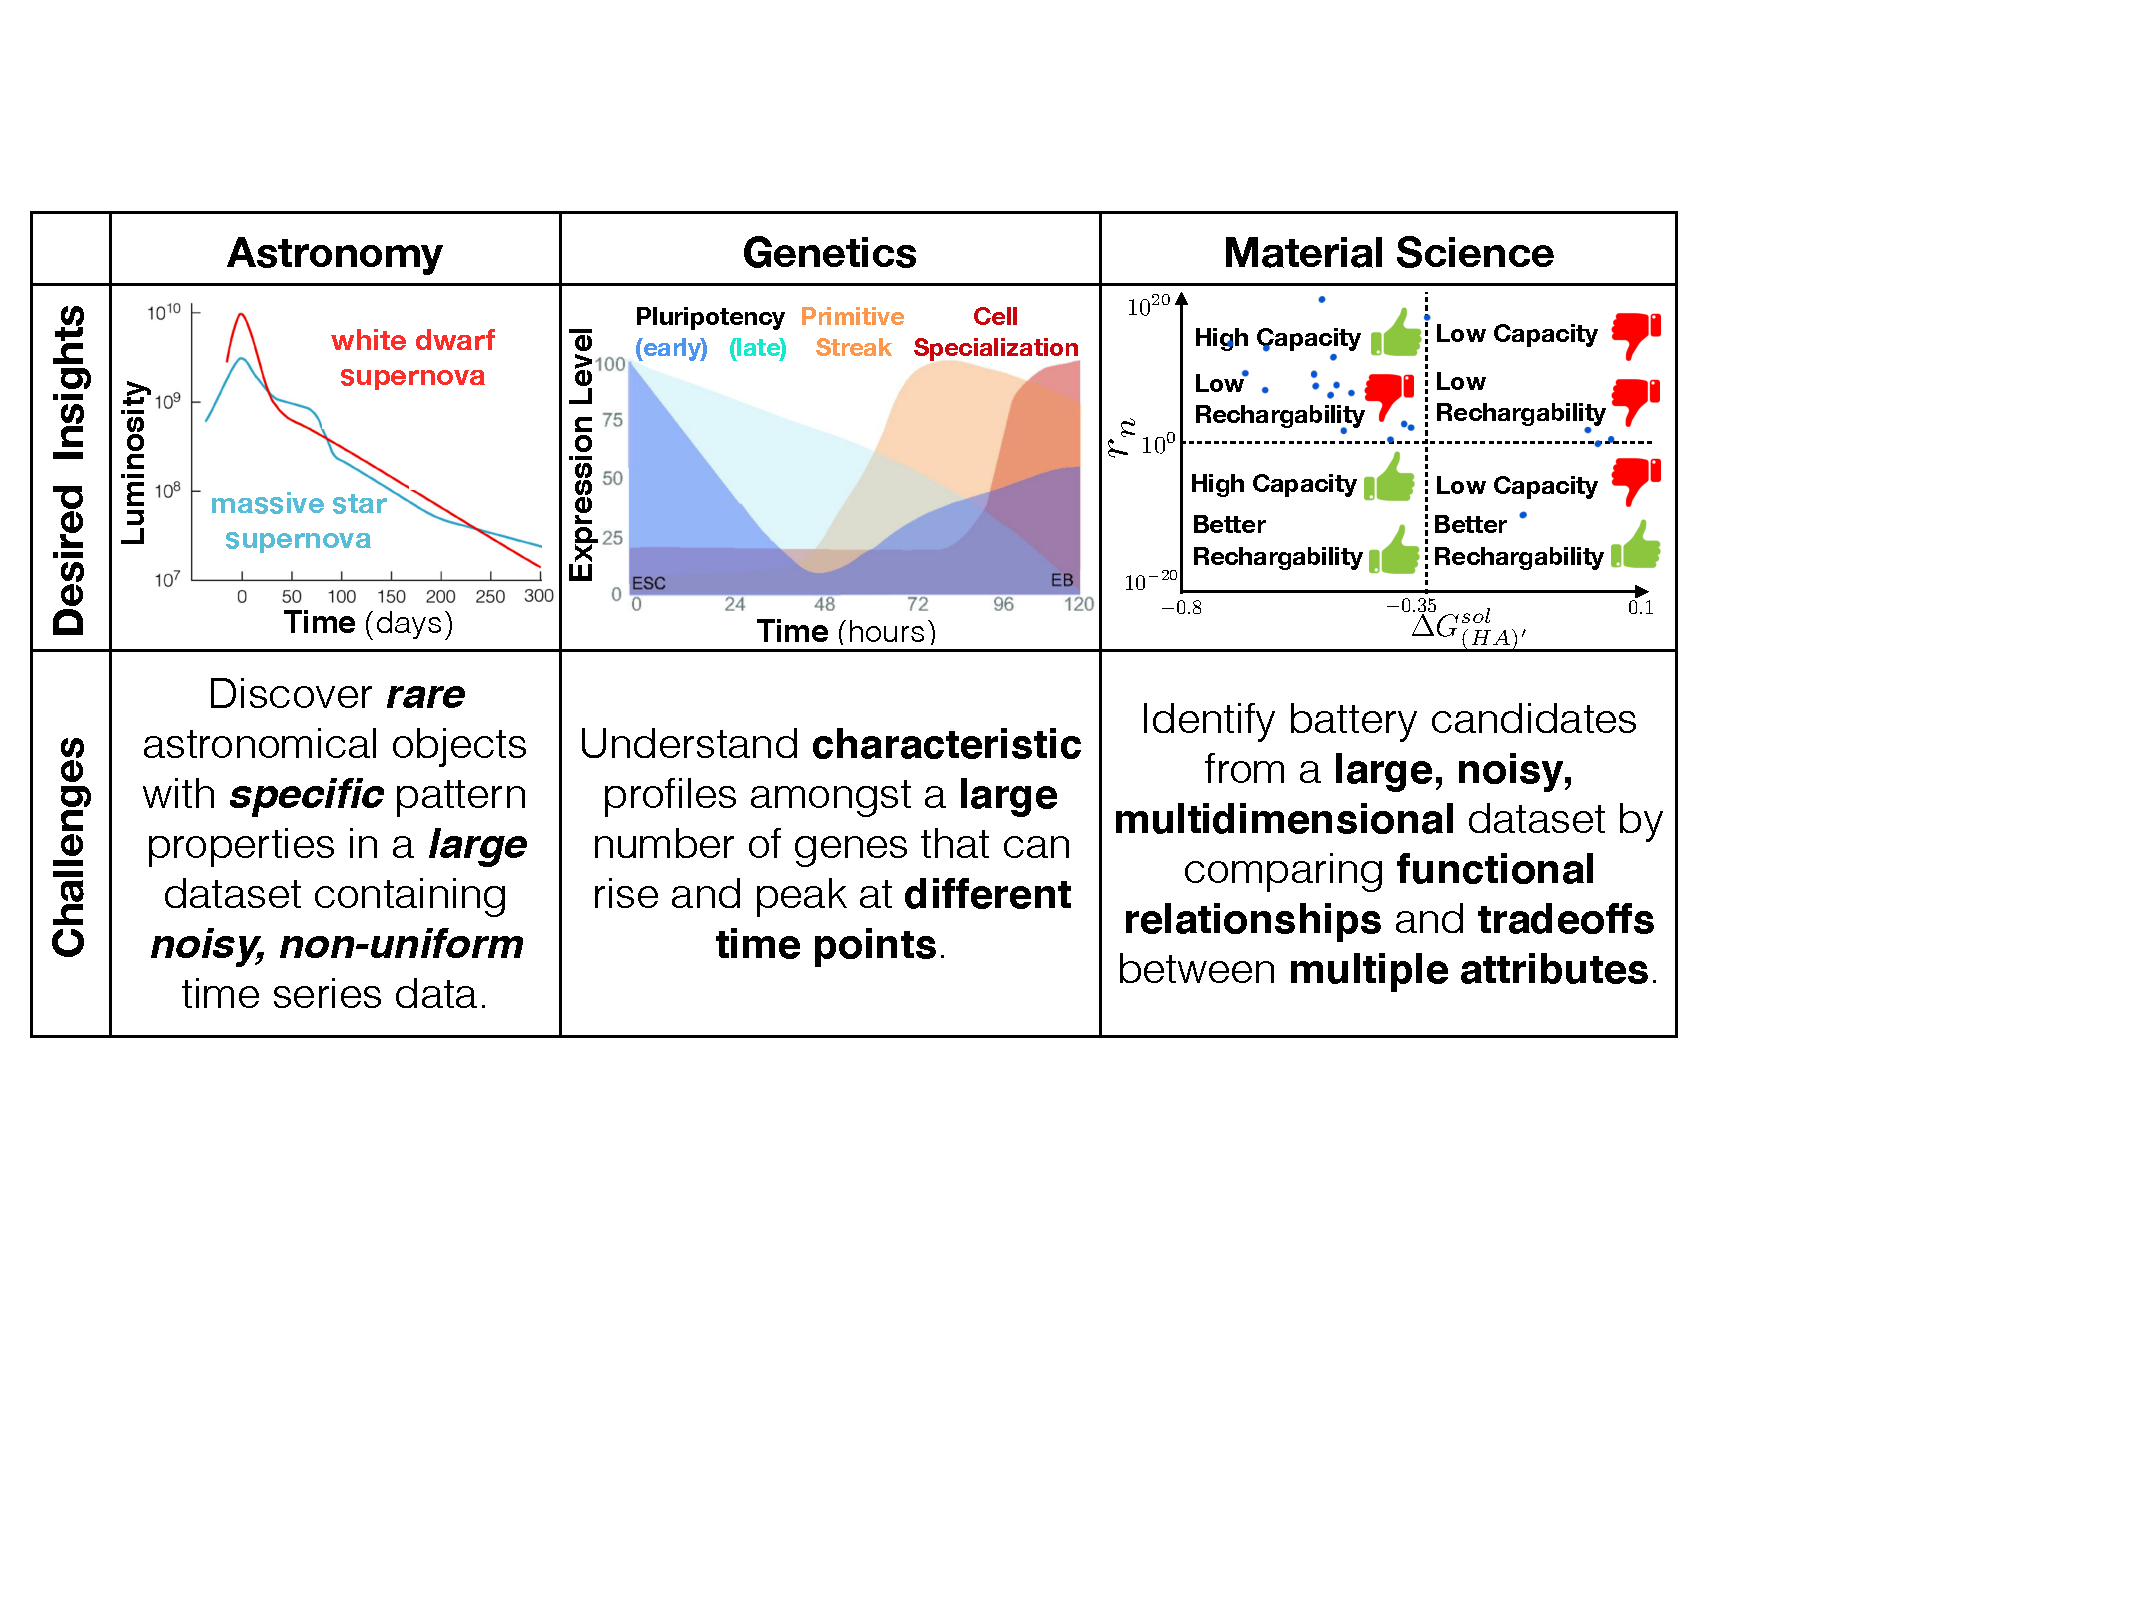
\includegraphics[width=\linewidth]{figures/science_goal.pdf}
	\caption{\change{Desired insights, problem and dataset challenges for each of the three application domains in our study.}}
	\label{science_goal}
	\vspace{-10pt}
\end{figure}
\par To study how various \change{VQSs} are used in practice,
we conducted a final evaluation study with nine participants
using our final VQS prototype to address their research questions
on their own datasets.
\change{During this 1.5-hour study}, participants were able to
gain novel scientific insights,
such as identifying a star with a transient pattern
that was known to harbor a Jupiter-sized planet
and finding characteristic gene expression profiles confirming the results of a related publication.\techreport{, and discovering that the dip in an astronomical light curve is caused by saturated imaging equipment overlooked by the existing error-detection pipeline.} \techreport{Participants also gain additional insights about their datasets, including debugging mislabeled features and uncovering erroneous data preprocessing procedure applied to a collaborator's dataset.}
\agp{Explain why these findings are important.}\dor{I think saying that planetary discovery is related to future colonization is a bit too much here.}
%that goes from a pattern in-the-head to a desired visualization

\par By analyzing the evaluation study results, we discovered that sketching a pattern for querying is often ineffective on its own. This is due to the fact that sketching makes the problematic assumption that users know the pattern that they want to sketch and are able to sketch it precisely. Instead, participants typically opted to combine sketching with other means of pattern specification---one common mechanism was to drag-and-drop a recommended pattern onto the canvas, and then modify it (e.g., by smoothing it out). However, most VQSs do not support these other mechanisms (as we argued earlier, they typically focus only on top-down sensemaking processes, without covering bottom-up and context creation), partially explaining why such systems have not been widely adopted in practice. %\change{Participants were, however, able to apply the two other sensemaking processes to gain novel scientific insights, such as identifying a star with a transient pattern that was known to harbor a Jupiter-sized planet, finding characteristic gene expression profiles confirming the results of a related publication, and discovering mislabelled features from a data preprocessing mistake.}
\par Further analysis of how participants
transition between different sensemaking processes
during analysis using a Markov model illustrated
how participants adopt a diverse set of workflows tailored
to their domains. We find that participants often construct analysis workflows focused around a primary sensemaking process, while iteratively interleaving their analysis with the two other processes. This finding points to how all three sensemaking processes, along with seamless transitions between them, are essential for enabling users to effectively use VQSs for data exploration.%For example, participants often center on a main sensemaking process, while interleaving variations with other two processes as they iterate on an analytic task.
%---including the construction of a Markov model---
\par To the best of our knowledge, our study is the \emph{first to holistically examine how VQSs can be designed to fit the needs of real-world
analysts and how they are actually used in practice}. \change{Working with participants from multiple domains (an uncommon practice for visualization design studies) enabled us to compare the differences and commonalities across different domains, thereby identifying general VQS challenges and requirements for supporting common analytical goals.} Our contributions include:
\begin{denselist}
\item a characterization of the problems addressable by VQSs through design studies with three different domains,
\item the construction of a taxonomy of functionalities within VQSs, as well as an articulation of the problem space that is amenable to VQSs, both grounded in participatory design findings,
\item \change{an integrative} VQS, \zvpp, \change{post participatory design} capable of facilitating rapid hypothesis generation and insight discovery,
\item study findings on how VQSs are used in practice, leading to the development of a novel sensemaking model for VQSs. %including the ineffectiveness of
%evaluation
% sketching and the ---- workflow
\end{denselist}
Our work not only opens up a new space of opportunities beyond the narrow use cases considered by prior studies, but also advocates common design guidelines and end-user considerations for building next-generation VQSs.
